\chapter{Superficies y variedades diferenciales}
  
  \section{Introducción: repaso en $\real^3$}
  
  En $\real^3$ tenemos puntos (dimensión 0), curvas (dimensión 1), superficies (dimensión 2) y abiertos (dimensión 3) sobre los que integrar en los que la imaginación resulta bastante útil. Pero... ¿qué pasa en $\real^N$? 
  
  Entonces en $\real^N$ tenemos objetos de dimensión $0,...,N$ sobre los que vamos a poder definir propiedades, integrales, etc.
  
\subsection{Cálculo del plano tangente en $\real^3$}  
  
  Repasamos la idea de que en $\real^3$ podíamos representar una superficie de varias maneras y cómo cálculabamos su plano tangente.
  \paragraph{Gráfica: $z=f(x,y)$} Dada una superficie como una gráfica, simplemente construíamos el vector normal al plano derivando parcialmente:
  
  \[ \vn = \left( \dpa{f}{x},\dpa{f}{y}, 1 \right) \]
  \paragraph{Parametrización}  Con una parametrización $\phi$ 
   	 \begin{align*}
  	 	\appl{\phi}{D\subset\real^2 &}{\real^3} \\     
     	\phi(u,v) &= (x(u,v),y(u,v),z(u,v))
     \end{align*}
  
     calculamos el plano tangente tomando los dos vectores directores y calculamos el normal al plano:
     \begin{gather*}
      	T_u = \left( \dpa{x}{u},\dpa{y}{u},\dpa{z}{u}\right)\\
      	T_v = \left( \dpa{x}{v},\dpa{y}{v},\dpa{z}{v}\right)\\
      	\overrightarrow{n} = T_u\times T_v\\
     \end{gather*}

     Nos podemos encontrar el problema de que $\overrightarrow{n} = \overrightarrow{0}$. Para evitar ese caso, estableceremos que el rango de la matriz de las 6 derivadas tiene que ser 2.
     
   \paragraph{Conjunto de nivel} Supongamos que nos dan una gráfica definida como un conjunto de nivel $F(x,y,z) = 0$ .
   
   Para calcular el plano tangente en este caso tenemos que $\overrightarrow{n} = \nabla F$. 
   
   Nos puede ocurrir que $F$ no sea derivable o que $\nabla F = \overrightarrow{0}$. Supongamos que sea diferenciable, ¿cómo preveer que puede salir? Para evitarlo, debemos forzar de nuevo que la matriz de las derivadas tenga rango máximo (en este caso 1).
   
   \subsection{Cálculo de la recta tangente en $ℝ^3$}
  
  Vamos a ver que pasa con las curvas en $\real^3$ y cómo calcular la recta tangente
  
  \begin{itemize}
   \item Parametrizada: \[\sigma(t) = (x(t),y(t),z(t))\]   
   \item Intersección de 2 superficies transversales, es decir,   
   \[C = \left\{\begin{array}{cc} F_1(x,y,z) &= 0\\ F_2(x,y,z) &= 0 \end{array} \right.\]   
   Posibles enemigos que nos podemos encontrar: superficies cuya intersección sea un plano. Si se da este caso, entonces tenemos que los vectores normales a las 2 superficies son paralelos. Para evitar esto, la matriz formada por los 2 vectores normales debe tener rango máximo.                                                                   
  \end{itemize}

 	Vemos claramente que las condiciones para poder calcular superficies tangentes llegan siempre a obligar a que la matriz tenga \textbf{rango máximo} (ver sección \ref{secThmRango}). A partir de aquí, podemos crear nuestra definición de subvariedad diferenciable:
 	
 	\section{Subvariedades diferenciables}
  
  \begin{defn}[Subvariedad\IS diferenciable]\label{defSubDif}
  Sea $M \subset \real^{M+N}$. Diremos que $M$ es una subvariedad diferenciable en $\real^{N+M}$ de dimensión $n$ y codimensión $k$\index{Codimensión} si y sólo si para todo punto $\ga$ existe un entorno abierto $U \subset \real^{N+K}$ con $\ga \in U$ de tal forma que $U \cap M = \{\gx\in U\tq F(\gx) = \gor{0}\}$ \textbf{para alguna función} $F\in C^1(U)$ con 
  
  \[\appl{F}{U\subset \real^{N+K}}{\real^K} \]
  
  cuya diferencial $DF$ tenga rango máximo (en este caso, rango $k$). De esta forma podremos expresar $U\cap M$ como 
  
  \[U\cap M = \left\{\begin{array}{cc}
                     F_1(x_1,...,x_{n+k}) = 0\\
                     F_2(x_1,...,x_{n+k}) = 0\\
                     \vdots\\
                     F_k(x_1,...,x_{n+k}) = 0
                    \end{array}\right.\] 
                    
  \end{defn}
  

Veamos ejemplos de si algunos objetos son variedades diferenciables o no:
\paragraph{1) Superficie en $\real^3$} 
  \[\appl{F}{U\subset\real^3}{\real}\]
  \[\{(x,y,z) \tq F(x,y,z) = 0\}\]
  En este caso tenemos $N=2, K=1$.
  La condición de rango nos dice que $\nabla F(\gx) \neq (0,0,0)$. Esto es, obliga a en cada punto existe un vector normal $\overrightarrow{n}$, exactamente la misma condición que habíamos visto antes.
  
  \begin{remark} Si tuviésemos la superficie expresada como gráfica de una función ($M = \{z = f(x,y)\}$) bastaría con tomar $F(x,y,z) = f(x,y)-z$. En este caso
  \[DF = \left(\dpa{f}{x},\dpa{f}{y},-1\right) \neq (0,0,0)\]
  Por lo tanto, las gráficas de funciones de 2 variables en $\real^3$ son siempre subvariedades (la condición de rango es gratuita).
  \end{remark}
  
\paragraph{2)  Curvas en $\real^3$}
  
  \[\sigma(t) = (x(t),y(t),z(t))\equiv S_1 \cap S_2 = \]
  \[= \{F_1(x,y,z) = 0\}\cap \{F_2(x,y,z) = 0\}\]
  Si tomamos $U\cap \sigma = \{(x,y,z)\in\real^3 \tq F_1 = 0 \y F_2 = 0\}$

  Siendo \[\appl{F}{U\subset\real^3}{\real^2}, N+K=3,K=2\]\[F(x,y,z) = (F_1(x,y,z),F_2(x,y,z))\]
  Veamos la condición de rango en este caso:
  \[rango \begin{pmatrix} \dpa{F_1}{x}&\dpa{F_1}{y}&\dpa{F_1}{z}\\\dpa{F_2}{x}&\dpa{F_2}{y}&\dpa{F_2}{z}\end{pmatrix}\]
  Para que el rango sea máximo, los vectores tienen que ser no paralelos, es decir, $S_1, S_2$ sean transversales, no paralelas. De nuevo, la misma condición que habíamos visto antes.
  
  \paragraph{3) Punto en $ℝ^k$}
  
  Podemos definir un punto de una manera un tanto rebuscada:
 \begin{gather*}
 \appl{F}{\real^K}{\real^K}\\
 \gx \rightarrow \gx - \ga
 \end{gather*}  
 
 En este caso, la subvariedad $M$ es nuestro punto $\ga$:
 
 \[M = \{\gx \in \real^K \tq F(\gx) = \gor{0}\} = \{\ga\}\]
 
 Tenemos $DF = Id $, que tiene rango máximo y por lo tanto $\{\ga\}$ es una subvariedad diferenciable (dimensión 0, codimensión $k$).
 
 \paragraph{4)} $\appl{F}{\Omega\subset\real^N}{0}$. En este caso tenemos codimensión $0$ y dimensión $N$.
 
\paragraph{5)}

  \begin{gather*}
  \appl{F}{\real^2}{\real}\\
   F(x,y) = x^3 - y^6 \\
  M = \{(x,y) \tq x^3-y^6 = 0\} \\
  DF = (3x^2-6y^5) \\
  DF(0,0) = (0,0)
  \end{gather*}
  La matriz diferencial tiene rango $0$ en el punto $(0,0)$. ¿Quiere esto decir que $M$ no es una subvariedad diferenciable en el 0?
  
  No. Lo que quiere decir que no hemos encontrado la función que cumpla las hipótesis. Podemos operar 
  \[M = \{x^3=y^6\} = \{x = y^2\}  = \{x-y^2 = 0\}\]
  
  Y vemos que si tomamos $G(x,y) = x-y^2$, esta función representa la misma subvariedad $M$, y $DG(x,y) = (1,2y)$ tiene rango 1 en el origen.
 
 
  \paragraph{6)}
  
  \[M = \{(x,y)\in \real^2 \tq x^2-y^2 = 0\}\]
  
	Definimos una función $F$:

	\[\appl{F}{\real^2}{\real}\]
	\[F(x,y) = x^2-y^2\]
  
  $DF = (2x,-2y)$. La condición de rango falla en $(0,0)$.
  
  Valoramos si este objeto no es una subvariedad o si tendremos que definir una función de una manera más inteligente, tal y como hicimos en el caso anterior.
  
  \begin{wrapfigure}{r}{0.4\textwidth}
	  \begin{center}
		  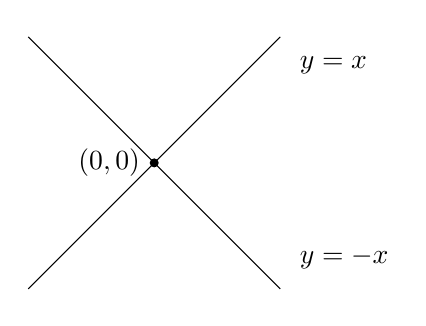
\begin{tikzpicture}
			  \draw (-1.6,-1.6) -- (1.6,1.6);
			  \draw (-1.6,1.6) -- (1.6,-1.6);
			  \node[circle, draw, fill=black, inner sep=1pt, label=left:{$(0,0)$}] at (0,0) {};
			  \node[label=above right:{$y=-x$}] at (1.6,-1.6) {};
			  \node[label=below right:{$y=x$}] at (1.6,1.6) {};
		  \end{tikzpicture}
		  \caption{Subvariedad $M = \{ y=x \cup y = -x \}$}
		  \label{figSubX}
	  \end{center}
  \end{wrapfigure}
  
  En este caso, vemos que $M = \{ y=x \cup y = -x \}$. No debería ser una subvariedad porque en el $(0,0)$ no es derivable (ver figura \ref{figSubX}). Intentaremos demostrarlo por reducción al absurdo.
  
  Supongamos que $M$ es una subvariedad. Entonces, según la definición (\ref{defSubDif})  existe un $U, (0,0) \in U$ y una aplicación  $\appl{G}{U\subset\real^2}{\real}$ con $U\cap M = \{G(x,y) = 0\}$. Entonces tendríamos que 
  
\[\rango DG(x,y) = 1, \forall(x,y) \in U \implies \rango \left(\dpa{G}{x},\dpa{G}{y}\right) = 1\]

Ahí tenemos dos casos, o bien que la primera componente no sea $0$ o que sea la segunda la que no es nula. Supongamos primero que $\dpa{G}{x}(0,0) \neq 0$. Podemos aplicar el Teorema de la unción implícita (\ref{TFImp}), que nos dice que podemos despejar $x = x(y)$. En este caso:

$U \cap M = \{x(y)^2-y^2 = 0\}$.

Si fijamos $y=\varepsilon$, entonces $x(\varepsilon) = \pm \varepsilon$ No es una función, lo que contradice el Teorema de la función implícita, y por lo tanto es imposible que $\dpa{G}{x}(0,0) \neq 0$. Análogamente, tampoco puede cumplirse que $\dpa{G}{y}(0,0) \neq 0$.

Hemos demostrado por lo tanto que no puede existir una función que defina esto como subvariedad diferencial. Este es el ejemplo de que cualquier objeto que tenga autointersección no puede ser subvariedad.

\paragraph{7)} $M = \{(x,y) \in \real^2 \tq x^2-y^2 = 0, y\ge 0\}$

Vamos a suponer que existe una función $F \in C^1$ que representa ese objeto (que viene definido por 2 condiciones). $M = \{F(x,y) = 0\}$ para alguna $F$.

Condición de rango: $\left(\dpa{F}{x},\dpa{F}{y}\right) \neq (0,0)$.
 Condición de rango: $\left(\dpa{F}{x},\dpa{F}{y}\right) = (0,0), x=y=0$.

 Vamos a ver si es subvariedad o no. En este caso intuimos que no debería serlo. Volvemos a demostrar por reducción al absurdo:

 Supongamos que $M$ es subvariedad, entonces $\exists G(x,y)$ tal que $\appl{G}{U\subset\real^2}{\real}, U \cap M = \{G(x,y) = 0\}$

 Supongamos $\displaystyle \dpa{G}{x}\neq 0$. Entonces tenemos \[ M\cap U = \{y(x)^2 - y^2 = 0\} \]

 Si fijamos $x=\varepsilon \implies y(x) = \abs{\varepsilon}$, pero esto quiere decir que $G \notin C^1$. De forma análoga con la segunda coordenada, vemos que $M$ no es una subvariedad.

\paragraph{8)} Nos quitamos el punto conflictivo del caso anterior, el $(0,0)$.

$N = \{(x,y)\in \real^2 \tq x^2-y^2 = 0, y>0\}$

La lógica nos dice que este caso si debería ser subvariedad diferencial:  la definición de la función es local, y siempre podremos encontrar un entorno que no incluya el 0, que es el punto problemático.

Comprobamos que efectivamente el rango de $\nabla F$ es máximo $\forall (x,y)\in \real^2$ y por lo tanto $M$ es una subvariedad.

\subsection{Subvariedades y parametrizaciones}
\paragraph{Ejemplo} Superficie en $\real^3$ parametrizada: $S = \{\Phi(u,v) = (x(u,v),y(u,v),z(u,v))\}$.

A la hora de trabajar con superficies parametrizadas, nos interesaría poder definir una especie de función inversa que nos permita hacer cambios en el plano y llevarlos a la superficie o al reves, pero... ¡tienen dimensiones distintas! La esperanza que nos queda es que la superficie parametrizada tiene dimensión 2, igual que el plano.

\begin{defn}[Homeomorfismo]
Sea $\appl{\Phi}{\Omega\subset\real^N}{\real^{N+K}}, \Omega$ abierto.

$\Phi$ es un \emph{homeomorfismo} sobre su imagen $\dimplies $ la restricción $\appl{\Phi}{\Omega}{\Phi(\Omega)}$ es continua y tiene una inversa continua,
es decir, \[\exists \appl{\Psi}{\Phi(\Omega)}{\Omega} \tlq 
\left\{ \begin{array}{cc} 
\Psi(\Phi(\gor{u})) = \gor{u}, &\forall \gor{u} \in \Omega\\ 
\Psi(\Phi(\gor{x})) = \gor(x), &\forall \gx \in \Phi(\Omega)
\end{array}\right.\]

\paragraph{Definición 1)}
Dado un $\displaystyle x_0 \in \Phi(\Omega) \implies \forall \varepsilon >0, \exists \delta>0 \tlq$ 

si $\begin{array}{lc}
\norm{\gx-\gor{x_0})} < \delta \implies \norm{\Psi(\gx)-\Psi(\gor{x_0})}<\varepsilon\\
\gx \in \Phi(\Omega)
\end{array}$

\paragraph{Definición alternativa de continuidad}
Si $\{X_n\}\subset\Phi(\Omega), \gor{X_n} \rightarrow \gor{x_0}\in\Phi(\Omega) \implies \Psi(\gor{X_n}) \rightarrow \Psi(\gor{x_0})$

\end{defn}

\subsubsection{Ejemplos}


\paragraph{Ejemplo 1}

\[\appl{\sigma}{[0,2\pi)}{\real^2}\]
\[t \rightarrow \sigma(t) = (cos(t),sen(t))\]

Inversa: $\Psi(x,y) = t$ ángulo de la representación en polares.

Vamos a estudiar el problema de la continuidad:

Tomamos $\{(X_n,Y_n)\}$ con $x^2+y^2 = 1 \tlq (x_n,y_n) \convs (1,0)$

Si $\Psi$ es continua, debe ser $\Psi(x_n,y_n) \convs (1,0) = 0$. En este caso no es continua porque:

Si tomamos \begin{align*}
P_n &= \left(cos\left(2\pi - \frac{1}{n}\right), sen\left(2\pi - \frac{1}{n}\right) \right)\\
P_n &\convs (1,0)\\
\Psi(P_n) &= 2\pi - \frac{1}{n} \convs 2\pi\neq\Psi(1,0)
\end{align*}

\paragraph{Ejemplo 2}

\[\appl{f}{(0,1)\subset\real}{\real^2}\]
\[t \rightarrow f(t) = (t,g(t)), \text{continua, con inversa continua}\]

Vamos a definir la  inversa:
\[P\in f(0,1) \implies P(x,g(x)) \text{Para algún } x\in(0,1)\]
$P = (x,g(x))$

\[\Psi(P) = t \in (0,1) \tlq f(t) = (x,g(x)) \implies t = x\]
Vamos a estudiar la continuidad:
\[\{P_n\} \subset f(0,1), P_n \rightarrow P \in f(0,1)\]
\[P_i = (x_i,g(x_i)), \text{ para algún } i \in (0,1)\]
\[P_n \convs P_0 \dimplies (x_n,g(x_n)) \rightarrow (x_0,g(x_0)) \implies x_n (= \Psi(P_n)) \rightarrow x_0 (=\Psi(P_0)) \]

\obs ¿La gráfica de una función es homeomorfismo sobre su imagen?
\paragraph{Ejemplo 3}
\[\appl{\sigma_3}{(0,4\pi)}{\real^2}\]
\[t \rightarrow \sigma(t) = (cos(t),sen(t))\]
No es inyectiva $\implies \nexists \Psi$.

\paragraph{Ejemplo 4: Circunferencia}
\[\appl{\sigma_4)}{(0,2\pi)}{\real^2}\]
\[t \rightarrow \sigma(t) = (cos(t),sen(t))\]
La diferencia con el ejemplo 1, es que es cerrado.

Hay que percatarse de que la tangente no es inyectiva, entonces... la inversa es algo más complicada que $\arctan$, así que vamos a definirla a trozos siguiendo el esquema de la figura \ref{imgCirc_2}.

\begin{figure}[hbtp]
\begin{center}
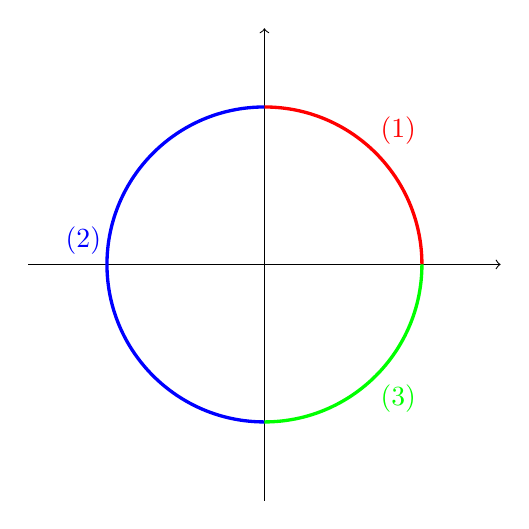
\begin{tikzpicture}[scale=1]
% Ejes
\draw[->] (-3,0) -- (3,0);
\draw[->] (0,-3) -- (0,3);

% Partes de la circunferencia
\draw[very thick,red] (2,0) arc (0:90:2);
\draw[very thick,blue] (0,2) arc (90:270:2);
\draw[very thick,green] (0,-2) arc(270:360:2);

% Etiquetas
\node[red] at (1.7, 1.7) {(1)};
\node[blue] at (-2.3, 0.3) {(2)};
\node[green] at (1.7, -1.7) {(3)};
\end{tikzpicture}
\caption{Circunferencia definida en tres trozos}
\label{imgCirc_2}
\end{center}
\end{figure}


\[\Psi(x,y) =
\begin{cases}
\arctan\left(\frac{y}{x}\right) & (x,y)\in 1\\
\arctan\left(\frac{y}{x}\right) + \pi & (x,y) \in 2\\
\arctan\left(\frac{y}{x}\right)+2\pi& (x,y) \in 3
\end{cases}
\]

Hay que estudiar la continuidad en $(0,-1)$ y en $(0,1)$.

\subparagraph{Continuidad en (0,1)}

Tomamos $\{P_n\} \rightarrow (0,1), P_n \in S_1$

Queremos probar que $\Psi(P_n) \rightarrow \Psi(0,1) = \frac{\pi}{2}$.

Ejercicio para el lector: 
Sucesiones que se acercan por la derecha o por la izquierda y comprobar que vale lo que tiene que valer.		

\paragraph{Ejemplo 5: Lemniscata}

\begin{figure}[hbtp]
\begin{center}
\begin{tikzpicture}[scale=2,declare function={
	lemnx(\x)=2.5*cos(\x) / ( sin(\x)^2+ 1);
	lemny(\x)=3*sin(\x) * cos(\x) / ( sin(\x) ^2 + 1;
	}]

% Ejes
\draw[->] (-3,0) -- (3,0);
\draw[->] (0,-2) -- (0,2);

% La curva
\draw[gray,domain=-90:270,samples=200] plot ({lemnx(\x)}, {lemny(\x)});

% Sucesión 1
\foreach \x in {-86,-82,...,-66}
\node[circle, red, draw,inner sep=2pt] at ({lemnx(\x)}, {lemny(\x)}) {};

% Sucesión 2
\foreach \x in {72,76,...,108}
\node[rectangle, blue, draw,inner sep=2pt] at ({lemnx(\x)}, {lemny(\x)}) {};

% Sucesión 3
\foreach \x in {242,246,...,266}
\node[diamond, orange, draw,inner sep=2pt] at ({lemnx(\x)}, {lemny(\x)}) {};

% Puntos t = 0, t=π
\node[label=above right:$t\eq 0$, draw, fill=white,circle, inner sep=2pt] at (2.5,0) {};
\node[label=above left:$t\eq \pi$, draw, fill=white,circle, inner sep=2pt] at (-2.5,0){};

% Flechas para indicar hacia donde va la t.
\foreach \x in {-45,44,134,224}
\draw[-angle 90] ({lemnx(\x)},{lemny(\x)}) -- ({lemnx(\x + 1)},{lemny(\x +1)});

% Etiquetas de las sucesiones.
\node[label={[red]below:(1)}] at ({lemnx(-66)},{lemny(-66)}) {};
\node[label={[blue]above:(2)}] at ({lemnx(72)},{lemny(72)}) {};
\node[label={[orange]above:(3)}] at ({lemnx(242)},{lemny(242)}) {};
\end{tikzpicture}
\caption{Curva Lemniscata}
\end{center}
\end{figure}

La parametrización es \[\sigma_5 (x(t),y(t)) = \left(\frac{\cos(t)}{\sin^2(t)+1},\frac{\sin(t)\cos(t)}{\sin^2(t)+1}\right), t\in \left(\frac{-\pi}{2},\frac{3\pi}{2}\right)\]

Al origen podemos acercarnos de distintas formas:

\begin{itemize}
\item Cuando $t \to - \frac{\pi}{2}$, nos acercamos por la sucesión 1 (desde abajo a la derecha).
\item Cuando $t \sim \frac{\pi}{2}$, nos acercamos por la sucesión 2 (la mitad de la curva, de arriba-derecha a abajo-izquierda).
\item Cuando $t \to \frac{3\pi}{2}$, nos acercamos por la sucesión 3 (desde arriba a la izquierda)
\end{itemize}

Sea $\{P_n\}\subset \sigma_5(t) \rightarrow (0,0)$.

Podemos tomar la sucesión $\{P_n\} = \{P_1,P_2,P_3,...\}$ cada uno en una región (1,2,3 ciclicamente).

\[\Psi(P_n) \begin{cases}
\in 3 & \text{ si }n \text{ es múltiplo de }3\\
\in 2 & \text{ si } n\equiv 2\ mod \ 3\\
\in 1 & \text{ si } n \equiv 1\ mod \ 3
\end{cases}\]

Por tanto $\nexists \displaystyle \lim_{n\rightarrow \infty} \Psi(P_n)$

\begin{remark} A pesar de que hemos demostrado que $\sigma$ es continua e inyectiva, esto no garantiza que la inversa sea continua.\end{remark}

\subsection{Parametrizaciones}

\paragraph{Objetivo} definir "parametrización".

\subparagraph{Ejemplo 1} Curva parametrizada en $\real^3$

$\Gamma = \{\sigma(t) = (x(t),y(t),z(t)), t \in (a,b)\}$

Queremos excluir:
\begin{itemize}
\item Picos (valor absoluto. FOTO) 

Basta con imponer: $\sigma \in C^1 \y (x',y',z') \neq (0,0,0)$

\item Auto-intersecciones o Lemniscata (que no se auto-intersecciona pero por poquito) 

Basta imponer $\sigma$ sea un homeomorfismo sobre su imagen.

\end{itemize}

\paragraph{Ejemplo 2} Superficies de parametrización en $\real^3$.

\[S = \{\Phi(u,v) = (x(u,v),y(u,v),z(u,v)), (u,v)\in D\}\]

Queremos evitar:

\begin{itemize}
\item Cono, tienda de campaña
$Rango \begin{pmatrix}
T_u \rightarrow\\
T_v \rightarrow
\end{pmatrix} = 2 \implies $ Podemos calcular plano tangente
\item Autointersección
Aquí sí tenemos rango máximo, asíque impondremos la condición de homeomorfismo sobre su imagen.
\end{itemize}

Ya tenemos todo lo necesario para definir parametrización:

\begin{defn}[Parametrización\IS local]
Diremos que $\appl{\Psi}{\omega \subset \real^N}{\real^{N+K}}, \Psi \in C^1(\omega)$, es una parametrización local $\dimplies \left\{ \begin{array}{c}
 rango D\Psi = n \text{ máximo}\\
 \Psi \text{ es un homeomorfismo sobre su imagen}
\end{array}\right.$
\end{defn}



\subsubsection{Repaso de coordenadas cilíndricas y esféricas.}
\paragraph{Ejemplos}

\index{Helicoide}\label{Helicoide}
El \textbf{helicoide} es una función $\Phi$ de dos variables, que crea una superficie helicoidal (escalera de caracol) en el espacio, tal que 

\begin{align*} \appl{\Phi}{\real^2 &}{\real^3} \\
 (s,t) &\longmapsto \Phi(s,t) = (s\cos t, s\sin t, t) \end{align*}
 
 \easyimg{CALII/Helicoide.png}{El helicoide}{lblHelic}

En general, una superficie parametrizada es una aplicación $\Phi$ de la siguiente forma:

\begin{align*} \appl{\Phi}{\Omega \subset \real^2 &}{\real^3} \\
 (s,t) &\longmapsto \Phi(s,t) = (x(s,t), y(s,t), z(y,t)) \end{align*}

\index{Paraboloide}
Por ejemplo, el \textbf{paraboloide} se puede definir como una superficie parametrizada \[\Phi(x,y) = (x,y,x^2+y^2)\].

\index{Cilindro}
Otro ejemplo es el \textbf{cilindro} de radio 2. Para parametrizarlo, usamos coordenadas polares de la siguiente forma:

\[ \Phi(t,z) = (2\cos t, 2\sin t, z)\;\;t\in [0, 2\pi],\;\; z\in \real \]

\index{Esfera}
Si queremos hacer la \textbf{esfera} de radio $R$, en la parametrización usamos dos parámetros (longitud y latitud)

\[ \Phi(\theta, \phi) = (R\sin\phi\cos\theta, R\sin\phi\sin\theta, R\cos\phi)\;\; \theta\in[0,2\pi],\;\;\phi\in[0, \pi] \]

\index{Toro}
El \textbf{toro} (una especie de flotador) se produce al girar una circunferencia de radio $R_1$ en el plano $XZ$ con el centro sobre el eje $X$ a $R_2$ del origen alrededor del eje $Z$.

\[ \Phi(\theta, \phi) = ((R_2+R_1\cos\phi)\cos\theta,(R_2+R_1\cos\phi)\sin \theta,R1\sin \phi)\;\; \theta, \phi \in [0, 2\pi] \]

 \easyimg{CALII/Toro.png}{Toro}{lblToro}
\paragraph{Parametrización de superficies de revolución}
\index{Superficie!de revolución}

Dada una función $\appl{f}{\real}{\real}$, la superficie de revolución que surge al rotar esta función sobre el eje z es la siguiente

\begin{align*} z(r,\theta) &= f(r) \\
x(r,\theta) &= r \cos \theta \\
y(r,\theta) &= r \sin \theta \end{align*} 

\paragraph{Coordenadas cilíndricas}
\index{Coordenadas!cilíndricas}
Dado un punto $P$, sus coordenadas cartesianas son $(x,y,z)$. Entonces, sus coordenadas cartesianas son $(r,\theta, z)$, donde $r\in [0,\infty)$, $\theta \in [0,2\pi]$ y $z\in \real$. La correspondencia es la siguiente:

\begin{align*}
x &=r \cos \theta \\
y &= r \sin \theta \\
z &= z
\end{align*}

Geométricamente, $z$ es la altura de $P$. Haciendo la proyección del punto sobre el plano $xy$, $r$ es la distancia de la proyección al origen y $\theta$ el ángulo del eje $X$ con la recta que une el origen y la proyección del punto.

\paragraph{Coordenadas esféricas}
\index{Coordenadas!esféricas}
Las coordenadas esféricas de un punto $P$ son $(\rho, \theta, \phi)$, donde $\rho \in [0, \infty)$, $\theta\in [0, 2\pi]$, $\phi \in [0, \pi]$. La correspondencia con coordenadas cartesianas es

\begin{align*}
x&=\rho \cos \theta \sin \phi \\
y&= \rho \sin \theta \sin \phi \\
z &= \rho \cos \theta
\end{align*}

Geométricamente, $\rho$ es la distancia de $P$ al origen, $\theta$ es el ángulo que forman el eje $X$ y la recta que une $P$ y el origen, y $\phi$ es el ángulo que forman el eje $Z$ y esa misma recta.

\paragraph{Usos de coordenadas esféricas y cilíndricas}

En las coordenadas cilíndricas, si mantenemos constante un parámetro y variamos los otros dos obtenemos varias superficies:

\begin{itemize}
\item Si $r$ constante, tenemos un cilindro. \index{Cilindro}
\item Si $\theta$ constante, tenemos un semiplano. \index{Semiplano}
\item Si $z$ constante, tenemos un plano horizontal. \index{Plano}
\end{itemize}

Lo mismo ocurre con las coordenadas esféricas:

\begin{itemize}
\item Si $\rho$ constante, tenemos una esfera. \index{Esfera}
\item Si $\theta$ constante, tenemos un semiplano.\index{Semiplano}
\item Si $\phi$ constante, tenemos un cono. \index{Cono}
\end{itemize}

\subsubsection{Ejemplos}

\subparagraph{Esfera en $\real^3$}
 $\Phi_{1,2}(x,y) = (x,y,\pm \sqrt{1-x^2-y^2})$. Esta \emph{"carta de parametrización"} nos deja sin definir el ecuador. Para ello tenemos que definir más \emph{cartas de parametrización} \index{Carta de parametrización}
 
 Estas cartas son expresando x,y en función de las otras 2. En total hacen falta 3 parametrizaciones.
 
 \subparagraph{Existe} otra manera de parametrizar, la proyección estereográfica.  
 \index{Proyección \IS estereográfica}

El dibujo de la proyección es:

\begin{tikzpicture} % "THE GLOBE" showcase
%Definición de constantes:
\def\R{2.5} % sphere radius
\def\angEl{15} % elevation angle
\def\angAz{-105} % azimuth angle
\def\angPhi{-40} % longitude of point P
\def\angBeta{19} % latitude of point P


%Ecuador
\DrawLatitudeCircle[\R]{0} 

\pgfmathsetmacro\H{\R*cos(\angEl)} % distance to north pole

\tikzset{xyplane/.estyle={cm={cos(\angAz),sin(\angAz)*sin(\angEl),-sin(\angAz),
                              cos(\angAz)*sin(\angEl),(0,0)}}}


\LongitudePlane[xzplane]{\angEl}{\angAz}
\LongitudePlane[pzplane]{\angEl}{\angPhi}
\LatitudePlane[equator]{\angEl}{0}

%% draw xyplane and sphere

\fill[ball color=white] (0,0) circle (\R); % 3D lighting effect
\draw(0,0) circle (\R);
\draw[xyplane] (-2*\R,-2*\R) rectangle (3.2*\R,2.8*\R);

\coordinate (O) at (0,0);

\coordinate[mark coordinate] (N) at (0,\H);
\coordinate[mark coordinate] (S) at (0,-\H);

\path[pzplane] (\angBeta:\R) coordinate[mark coordinate] (P);
\path[pzplane] (2.75*\R,\R) coordinate (PE);
\path[xzplane] (0,0) coordinate (XE);
\path (PE) ++ (0,0) coordinate (Paux); % to aid Phat calculation
\coordinate[mark coordinate] (Phat) at (intersection cs: first line={(N)--(P)},
                                        second line={(S)--(Paux)});

\coordinate[mark coordinate] (P1) at (-2,-5/3);

\coordinate[mark coordinate] (P2) at (4,2/3);

\DrawLatitudeCircle[\R]{-1} % equator
\draw[xyplane,<->] (4*\R,0) node[below] {$u$} -- (0,0) -- (0,2.4*\R)
    node[right] {$v$};
\draw[->] (0,-\H) -- (0,1.6*\R) node[above] {$z$};

\draw[dashed] (P) -- (N) +(0.3ex,0.6ex) node[above left] {$\mathbf{N}$};
\draw (P) -- (Phat) node[above right] {$\mathbf{\hat{P}}$};
\path (S) +(0.4ex,-0.4ex) node[below] {$\mathbf{S}$};
\draw[->] (O) -- (P) node[above right] {$\mathbf{P}$};
\draw[blue] (P1) -- (P2) node[below right] {$\mathbb{X}\left(u,\frac{u-2}{3}\right)$};	

\path (P1) node [above left] {$\left(-2,\frac{-5}{3},0\right)$};
\path (P2) node [left] {$\left(4,\frac{2}{3},0\right)$};

\draw[red,name=lineP1N] (P1) -- (N);
\draw[red,name=lineP2N] (P2) -- (N);


\end{tikzpicture}


La imagen formada será la circunferencia que contenga la intersección (que ya no he sabido dibujar) de cada línea roja con la esfera y las 2 intersecciones (que tampoco he sabido dibujar) de la recta azul que es $\mathbb{X}\left(u,\frac{u-2}{3}\right)$.

 
 
 \[(u,v) \in \real^2 \rightarrow (u,v,0) \rightarrow r\equiv (0,0,R) + t(u,v,-R) = (tu,tv,R(1-t)\]
 Imponiendo $\underbrace{P}_{r(t_0)} \equiv r\cap S$ tenemos: \[(t_0u)^2+(t_0v)^2 + R^2(1-t)^2 = R^2 \rightarrow ... \rightarrow t_0 = \frac{2R^2}{u^2+v^2+R^2}\]
 
 Conclusión: \[P = (tu,tv,R(1-t) = \frac{2R^2}{u^2+v^2+R^2}u,\frac{2R^2}{u^2+v^2+R^2}v,\frac{R(u^2+v^2-R^2)}{u^2+v^2+R^2} = \Phi(u,v)\].
 
 Vemos que $\Phi\in C^1, \Phi(\real^2) = S_R-\{(0,0,R)\}$ ¿Es una parametrización?
 
 Hay que comprobar \begin{itemize}
 \item rango $D\Phi$ máximo. (Se deja como ejercicio para el lector)
 \item $\Phi$ es homeomorfismo sobre su imagen, es decir, ¿Existe una inversa continua? 
 
 \emph{Inversa}
 Dado $(x,y,z)$ queremos despejar $(u,v)$.
 
 Idea: $(u,v,0)$ es la intersección de la recta que unie $(x,y,z)$ con $(0,0,R)$ y el plano $z=0$.
 
 Recta: $s(t) = (tx,ty,R+t(z-R))$.
 
 Punto de corte con el plano $z=0$: El punto de corte tendrá coordenada tercera = 0, es decir: 
 $R+t(z-R)$
 
 Buscamos $t_0$ tal que $R+t_0(z-R)=0 \dimplies t_0=\frac{R}{R-z}$.
 
 Sustituyendo en la recta obtenemos: $u = t_0x, v=t_0y$
 
 Si calculamos $\Phi^{-1}(x,y,z) = \left(\frac{Rx}{R-z},\frac{Ry}{R-z}\right)$. Esta inversa es continua en $Img(\Phi(\real^2)) \equiv \{Esfera - \{(0,0,R)\}\}$  (El punto (0,0,R) no está incluido, por definición, en la imagen).
 
 \end{itemize}
\subsection{Teoremas de las subvariedades}
\begin{theorem}
Los siguientes enunciados son equivalentes:
\begin{itemize}
\item[1] $M$ es una subvariedad diferenciable n-dimensional en $\real^{N+K}$. \label{eq_1}
\item[2] $\forall \gor{a} \in M $ existe una parametrización local $\appl{\Phi}{\omega\subset \real^N}{\real^{N+K}}$ con $\gor{a}\in \Phi(\omega)$\label{eq_2}
\item[3] $\forall \gor{a} \in M$ existe un abierto $V\in \real^{N+K}, \gor{a}\in V$ y una aplicación 
\label{eq_3}
\[\appl{\Psi}{V}{\real^{N+K}}, \Psi\ difeomorfismo \tlq \Psi = (\Psi_1,...,\Psi_n,\Psi_{n+1},...,\Psi_{n+k})\]
Si $\gx \in V\cap M \implies$
\[\Psi_{n+1}(\gx) = ... = \Psi_{n+k}(\gx) = 0\]
\end{itemize}
\end{theorem}
 
 \paragraph{Observación 1:} En \ref{eq_2}.2, llamaremos carta local al conjunto definido por la fórmula y el dominio, $(\Phi,\omega)$. El conjunto de todas las cartas locales que definen una subvariedad se llama Atlas.
 
 \subparagraph{Ejemplo:} 
 
 La proyección estereográfica tiene 2 cartas, la del polo norte (que excluye ese punto) y la del polo sur.
 
 \paragraph{Observación 2:} $\ref{eq_1}.1 \dimplies \ref{eq_2}.2$. Si tenemos una grádica dada como conjunto de nivel la podemos parametrizar (y viceversa).
 
\begin{defn}[Difeomorfismo]
$\Psi$ es un difeomorfismo $\dimplies \Psi\in C^1,\exists \Psi^{-1}, \tlq \Psi^{-1}\in C^1$
\end{defn}
 


\begin{proof}
Esquema: $1\implies 2, 2\implies 3, 3 \implies 1$

\paragraph{1 $\implies$ 2\\}

Sea $\ga \in M, \exists U\subset\real^{N+K}$ abierto con $\ga \in U$ y una función $\appl{F}{U\subset \rnk}{\rk}, F\in C^1(U), \tlq U\cap M = \{\gx \in U\tq F(\gx) = \gor{0}\}$. Además $DF$ tiene rango máximo (K). 

Queremos demostrar que existe una parametrización $\Phi$.
\subparagraph{Permutando} el orden de las variables, suponemos que el menor de orden $K$ con determinante no nulo corresponde con las $K$ últimas variables. 

Por el teorema de la función implícita, $F(x_1,...,x_n,x_{n+1},...,x_{n+k}) = \gor{0}$, con $x_{n+1},...,x_{n+k}$ despejable en función de las $\{x_i,i=1,...,n\}$ en un entonro de $\gor{a}$.

Es decir: existen $\omega\subset \real^N, \omega'\subset\rk$ abiertos tales que $\gor{a}\in \omega \times \omega'$ y una función $\appl{g}{\omega\subset\real^N}{\omega'\subset\rk}$ de manera que
$$\left\{\begin{array}{c}
g(a_1,...,a_n) = (a_{n+1},...,a_{n+k})\\
F(\gx,g(\gx)) = \gor{0}, \forall \gx \in \omega\end{array}\right.$$

Idea: la parametrización es $\Phi (\gx) = (\gx,g(\gx))$

Vamos a comprobar las condiciones:
\begin{itemize}
\item $\Phi \in C^1$. Por el teorema de la función implícita, tenemos que $\Phi$ es diferenciable (porque $F$ y $g$ lo son).
\item \[D\Phi = ... = 
\begin{pmatrix}
Id_{n \times n}\\
\hline
Dg
\end{pmatrix}\] con rango máximo.
\item ¿Homeomorfismo sobre su imagen? $(x,y)\in M$ en un entorno de $\ga \in \omega\times\omega'$ En ese entonrno $y=g(\gx)$.
\end{itemize}
Es decir, $(x,y) = (x,g(x)) \xrightarrow{\Phi}) \gx \xrightarrow{\Phi^{-1}} (x,g(x)) = (x,y) $. También $\inv{\Phi}(x,y) = x, \forall(x,y)\in (\omega\times\omega') \cap M$ Continua.


\paragraph{2 $\implies$ 3} Vamos a emplear un argumento como el de la demostración del segundo teorema del rango. \ref{TR2}

Buscamos: 
\begin{align*}
\appl{\Phi}{\rnk}{\rnk} \tlq \Phi(V\cap M) = (\ast &,0)\\
&\uparrow\\
k \text{ últimas coor} & \text{denadas}
\end{align*}
Siendo $\Phi$ un difeomorfismo.

\paragraph{Sabemos:} existe una parametrización local $\appl{\Psi}{\real^N}{\rnk}$.
\begin{itemize}
\item $D\Psi$ rango máximo.
\item $\Psi$ homeomorfismo sobre su imagen.
\end{itemize}

\subparagraph{Idea:} Completar el número de variables

Definimos 
\begin{align*}
\appl{\alpha}{\omega\times\real^K \subset \real^N\times\real^K}&{\real^N\times\real^K}\\
(\gor{u},\gor{v})\longrightarrow &\alpha(\gor{u},\gor{v}) = \Psi(\gor{u}) + (\gor{0},\gor{v})\\
\gor{u} \in \real^N,\gor{v} \in \real^K, \Phi(\gor{u})\in \real^{N+K}
\end{align*}

\paragraph{Paso 2)} Aplicar el teorema de la función inversa (\ref{TFInv}) a $\alpha$.

\[D\alpha =
\left(
	\begin{array}{c|c}
		D\Psi_k  \rightarrow & 0\\
		\hline
		D\Psi_{n+i}  \rightarrow & I
	\end{array}
\right)
\]
Con $1\leq i \leq k,1\leq k \leq n$.

Por hipótesis, $rango(D\Psi)$ máximo. $\implies \exists \alpha^{-1}$.

\paragraph{Paso 3:} Comprobar que $\inv{\alpha}$ verifica las condiciones que buscamos.

Podría darse el caso de que en el conjunto $V\cap M$ hubiera 2 "trozos" de la subvariedad M, con lo que $\alpha$ no funcionaría bien. La condición de la parametrización eliminaba este caso.

Falta comprobar la condición de difeomorfismo, que se da porque... ¿porqué?

\paragraph{3 $\implies$ 1}

\textbf{Sabemos:} Existe un difeomorfismo $\Psi$.

\textbf{Buscamos:} $\appl{F}{W\subset \rnk}{\real^K} \tlq \displaystyle \left\{\begin{array}{c}
M\cap W = \{F(\gx) = \gor{0}\}\\
rango(DF) = k \text{ (máximo)}
\end{array}\right.$

Tomamos $F(\gx) = (\Psi_{n+1}(\gx),...,\Psi_{n+k}(\gx))$

Entonces: $M\cap V = \{ \gx \tq F(\gx) = \gor{0}$.

Tenemos $DF = \begin{pmatrix}
D\Psi_{n+1} \rightarrow\\
\vdots\\
D\Psi_{n+k} \rightarrow
\end{pmatrix}$

$Rango(DF) = k$ por tener $\det D\Psi \neq 0$ por hipótesis.

\end{proof}

\paragraph{Consecuencias:}

\subparagraph{1)}
Si $M$ es una variedad diferenciable de dimensión $N$ en $\rnk$, entonces, reordenando las variables puede escribirse \textbf{localmente} como la gráfica de una función $C^1, \underbrace{M\cap U}_{(*)} = \{(\gx,g(\gx))\}$

$(*) \implies$ un trozo de la variedad.


\subparagraph{2)}

\begin{theorem}
Sea  $\appl{\gamma}{\omega\subset\real^N}{\rnk}, \gamma \in C^1, rg(D\gamma) = max, \gamma(\omega)\subset M$ subvariedad de dim n.

\textbf{Entonces:} $\gamma$ es una parametrización local.	
\end{theorem}

\textbf{Aplicación:} Si existe $\gamma \in C^1, rg(D\gamma) = n, \gamma(\omega)\subset M \ y \ \gamma
$ no es homeomorfismo sobre su imagen $\implies$ \textbf{M} no es subvariedad.

Pregunta: Verdadero o Falso:

¿Con encontrar una aplicación que no sea homeomorfismo basta para asegurar que M no es subvariedad?

\paragraph{3)\\}

No vamos a probar el siguiente teorema por que no nos apetece xD

\begin{theorem}
Sea M subvariedad diferenciable n-dimensional en $\rnk$.

Sean $\appl{\Phi_1}{U_1}{M} \ y \ \appl{\Phi_2}{U_2}{M}$ dos parametrizaciones locales con $\Phi_1(U_1)\cap \Phi_2(U_2)\neq \emptyset$

\textbf{Entonces:} $\appl{\inv{\Phi_1}\circ \Phi_2}{\real^N}{\real^N}, con \inv{\Phi_1}\circ \Phi_2 \in C^1$. Análogamente para $\inv{\Phi_2}\circ\Phi_1$
\end{theorem}

\section{Espacios tangentes}

Sea $M$ subvariedad n-dimensional en $\rnk$.

$T_{\gor{a}}M \leadsto$ espacio tangente a M en el punto $\gor{a}\in M$

Pero... ¿qué es un hiperplano tangente? El concepto no es tan simple como un plano tangente. El espacio tangente será el conjunto de todos los vectores tangentes a cada una de las curvas contenidas en la superficie. A partir de aquí buscaremos una forma más eficiente de construirlo (porque es imposible calcular todas y cada una de las curvas contenidas en la superficie).

\begin{defn}[Vector tangente]
Si $\gx \in \rnk$ es tangente a M en $\gor{A} \in M \dimplies \exists \appl{\sigma}{(-1,1)}{\rnk}, \sigma \tlq \left\{\begin{array}{lc}
\sigma(t) \in M, \forall t\in (-1,1)\\
\sigma(0) = \gor{a}\\
\alpha'(0) = \gor{v}
\end{array}\right.$
\end{defn}
\begin{defn}[Espacio tangente]
\[T_aM \equiv \{ \gor{v} \in \rnk \tq \gor{v} \text{ es tangente a M en }\gor{a}\}\]
\end{defn}

\obs Cualquier curva de la variedad la podremos ver como una curva en la proyección (con una parametriazación construida cuidadosamente)

\begin{theorem}
Sea $M$ subvariedad en $\real^M$, $N$ subvariedad en $\real^N$.
\[\appl{f}{\Omega\subset\real^M}{\real^N}, \tlq f(\Omega\cap M) \subset N, f\in C^1\]

Sea \[\left.\begin{array}{lc}
\gor{a} \in \Omega\cap M \\ 
\gor{v} \in T_aM
\end{array}\right\} 
\implies Df(\gor{a})\gor{v} \in T_{f(\ga)}N\]
\end{theorem}

Es decir, si tenemos una parametrización, la diferencial lleva tangentes en tangentes.

\begin{proof}
Sea $\gor{v} \in T_{\ga} M$
Entonces $\exists \appl{\alpha}{(-1,1)}{M} \tlq \left\{\begin{array}{c}
\alpha(0) = \ga\\
\alpha'(0) = \gor{v}
\end{array}\right.$
Tomamos $\beta = f \circ \alpha$ curva sobre $N$ 

tal que $\left\{\begin{array}{lc} \beta(0) = f(\alpha(0)) = f(\ga)\\ 
\beta'(0) = Df(\alpha(0))\cdot \alpha'(0) = Df(\ga)\gor{v}\end{array}\right.$ (Aplicando la regla de la cadena sin más.)
\end{proof}


\subsection{Caracterizaciones del espacio tangente}
\textbf{Caracterización 1)}
\begin{theorem}

$M$ subvariedad n-dimensional en $\rnk$. $\ga \in M$

Entonces:

\begin{itemize}
\item $T_{\ga}M$ es un espacio vectorial n-dimensional
\item $M$ definida como $\{F = 0\}$. Entonces $T_{\ga} M = \ker(DF(\ga))$
\end{itemize}
\end{theorem}

\begin{proof}
$U\cap M =\{ \gx \in \rnk \tq F(\gx) = \gor{0}\}$ para alguna $\appl{F}{\rnk}{\real^N}, rg(DF) = max$

\[\appl{F}{U\cap M}{\gor{0}}\]

Entonces: $DF(\ga)$ lleva $T_a M$ al espacio $T_0\{\gor{0}\}$

Es decir: $DF(\ga)\gor{v} = \gor{0}, \forall \gor{v}\in T_{\ga} M$

Esto demuestra $T_{\ga} M \subset \ker DF(\ga)$

Como el rango es máximo, sabemos que $\ker(DF(\ga))$ tiene dimensión $n$.

La idea a aplicar es encontrar $n$ vectores independientes en ese espacio tangente ¿Cómo vamos a encontrarlos? En el espacio de los parámetros tenemos n rectas independientes (los n ejes de coordenadas)

La parametrización nos lleva esas $n$ rectas en $n$ curvas. 

Por el teorema anterior, la diferencial lleva tangentes en tangentes, es decir, aplicando la diferencial a los vectores directores de las $n$ rectas encontramos los vectores tangentes a las $n$ curvas. 

¿Cómo podemos saber que esos vectores son independientes? Porque la diferencial tiene rango $n$.

Acabamos de demostrar  $\ker DF(\ga) \subset $\{ espacio vectorial de dimensión n\} 

Si $T_{\ga} M$ contiene un espacio vectorial de dimensión $n$ y está contenido por el núcleo (espacio vectorial de dimensión $n$).
\end{proof}

\paragraph{Caracterización 2)}
\begin{corol}
\label{CaractSubv_2}
$M$ dada por una parametrización $\Phi$ tal que $\Phi(\gor{u_0}) = \ga$ 

Entonces $T_{\ga} M = \img D\Phi(\gor{u_0})$

\end{corol}


El teorema y el corolario son las 2 caracterizaciones del espacio tangente.

Pero también podemos definir el espacio tangente con una tercera caracterización:

\paragraph{Caracterización 3)} Como gráfica. Sea $\appl{f}{\real^k}{\real^{n-k}}$

\[M\equiv \left\{(\gu,f(\gu)),\begin{matrix}
(\gu,f(\gu))\in \rnk\\
\gu \in \Omega\subset\real^N\\
 \appl{f}{\real^N}{\real^K}\end{matrix}\right\} \]

Salvo reordenación de las variables.

Sea $p=(\ga,f(\ga))$ el punto en el que queremos calcular el hiperplano tangente a $M$.

La caracterización será
\[T_p(M) = \{(\gu,v)\in\real^k\x\real^{n-k} \tq v = df(a) \gu\}\]

\obs la otra alternativa es definir la subvariedad como $M = \{(\gu)\in\real^k \tq f(\gu) = f(\ga)$

\begin{defn}
$M\subset\rnk$ subvariedad n-dimensional, $\ga \in M$

\begin{itemize}
\item Espacio tangente $T_{\ga}M$
\item Hiperplano tangente $T_{\ga}$ "trasladado" al punto $\ga$
\[\{\gx \in \rnk \tq \gx-\ga \in T_{\ga}M\}\]
\item Hiperplano normal $\equiv \{\gx\in\rnk \tq \gx -\ga \in (T_{\ga}M)^{\bot}\} = \{\gx \in \rnk \tq \pesc{\gx-\gor{a},\gor{v}} = 0, \forall \gor{v}\in T_{\ga}M\}$. El hiperplano normal es k-dimensional.
\end{itemize}
\end{defn}


\paragraph{Ejemplos:}

\subparagraph{1)}

$ M = \{(x,y) \in \real^2 \tq x^2+y^2 = 1\}$.

\textit{Comprobación previa} Es una subvariedad porque...


Vamos a calcular \[T_{(a,b)}M = \ker \{\begin{pmatrix} 2x & 2y \end{pmatrix}\} =\]
\[ \{(u,v) \tq \begin{pmatrix}
2a & 2b
\end{pmatrix}\begin{pmatrix}
u\\v
\end{pmatrix} = 0\} = ... =  \{(u,v)\in \real^2 \tq \pesc{(a-0,b-0),(a,b)-(u,v)} = 0\].

El espacio tangente es el formado por todos los vectores perpendiculares al radio.

\subparagraph{Ejemplo 2: Toro (donut) en $\real^4$}

\[M = \{ (x,y,z,t)\in \real^4 \tq x^2+y^2 = 1, z^2+t^2 = 1\}\]
Vamos a calcular: $T_{(1,0,0,1)}M$

\textbf{Comprobación previa}...

Tenemos definida la variedad de forma implícita: $M = \{F = 0\}$ donde \[F(x,y,z,t) = (x^2+y^2-1,t^2+z^2-1)\]

\[DF = \begin{pmatrix}
2x&2y&0&0\\
0&0&2z&2t
\end{pmatrix}\]

En este caso tenemos $rg(DF) = 2, \forall (x,y,z,t)\in \real^4$. (El único punto que podría dar rango 0 es el origen, que en este caso no pertenece a la subvariedad)

Vamos con el espacio tangente:

\[T_{(1,0,0,1)}M = \ker DF (1,0,0,1) = \ker \begin{pmatrix}
2&0&0&0\\
0&0&0&2
\end{pmatrix} =\]
\[ \{ (\alpha_1,\alpha_2,\alpha_3,\alpha_4) \in \real^4 \tq \begin{pmatrix}
2&0&0&0\\
0&0&0&2
\end{pmatrix} \begin{pmatrix}
\alpha_1\\
\alpha_2\\ \alpha_3\\ \alpha_4
\end{pmatrix} = \begin{pmatrix}
0 \\
0
\end{pmatrix}\} \implies \left\{\begin{array}{cc}2\alpha_1 &= 0\\ 2\alpha_4 & =0\end{array}\right.\]

Hiperplano tangente:

\[
\begin{pmatrix}
1\\0\\0\\1
\end{pmatrix}
+ \alpha_2 \begin{pmatrix}
0\\1\\0\\0 	
\end{pmatrix}
+ \alpha_3
\begin{pmatrix}
0\\0\\1\\0
\end{pmatrix}, \alpha_2,\alpha_3 \in \real
\]

Y el hiperplano normal:

\[
\begin{pmatrix}
1\\0\\0\\1
\end{pmatrix}
+ \mu \begin{pmatrix}
1\\0 \\0\\0 	
\end{pmatrix}
+
\lambda
\begin{pmatrix}
0\\0\\0\\1
\end{pmatrix}, \lambda,\mu \in \real
\]

¿Una posible parametrización de esto?

\begin{align*}
\Phi : D \subset \real^2 \longrightarrow &\real^4\\
(u,v) \longrightarrow &\Phi(u,v) = (x,y,z,t) = \left(cos(u),sen(u),cos(v),sen(v)\right)\\
(u,v)\in (-\pi,\pi)\times(0,2\pi)
\end{align*}

¿¿Por qué $(u,v)\in (-\pi,\pi)\times(0,2\pi)$ y no $(u,v)\in (0,2\pi)\times(0,2\pi)$??

Porque el punto que tenemos $(1,0,0,1) \notin \img$. 

Vamos a calcular la el hiperplano tangente. Como tenemos una parametrización, calcularemos la imagen de la diferencial (\ref{CaractSubv_2})
\[T_{(1,0,0,1)}M = \img D\Phi\left(0,\frac{\pi}{2}\right)\]
\[D\Phi = \begin{pmatrix}
-sen(u) & 0\\
cos(u) & 0\\
0 & -sen(v)\\
0&cos(v)
\end{pmatrix}\]
\[D\Phi\left(0,\frac{\pi}{2}\right) = \begin{pmatrix}
0&0\\1&0\\0&-1\\0&0
\end{pmatrix}\]

Entonces el hiperplano tangente es:

\[\begin{pmatrix}
1\\0\\0\\1
\end{pmatrix} + u \begin{pmatrix}
0\\1\\0\\0
\end{pmatrix}
- v \begin{pmatrix}
0\\0\\1\\0
\end{pmatrix}
\]

Lógico y normal que nos de el mismo hiperplano tangente si estamos trabajando con el mismo objeto (desde una parametrización o desde un conjunto de nivel). ¿Cierto y verdad que sí?

\paragraph{Ejemplo 3: El toro en $\real^3$}
\index{Toro}

El \textbf{toro} (una especie de flotador) se produce al girar una circunferencia de radio $R_1$ en el plano $XZ$ con el centro sobre el eje $X$ a $R_2$ del origen alrededor del eje $Z$.

\[ \Phi(\theta, \phi) = ((R_2+R_1\cos\phi)\cos\theta,(R_2+R_1\cos\phi)\sin \theta,R1\sin \phi)\;\; \theta, \phi \in (0, 2\pi) \]

\easyimg{CALII/Toro.png}{Toro}{lblToro2}

¿Es $\Phi$ una parametrización? 
\begin{itemize}
\item Opción 1: Comprobar homeomorfismo sobre la imagen
\item Opción 2: Aplicar el teorema. Si el toro es una subvariedad $\implies \Phi$ parametrización.
\end{itemize}

Vamos con la opción 1:
\[\Phi(\alpha,\theta) = (x,y,z)\]
\[¿(\alpha,\theta) = \Phi^{-1} (x,y,z)?\]
\[z = rsen(\alpha) \implies \alpha = arcsen\left(\frac{z}{r}\right)\]
\[\frac{y}{x} = tg(\theta) \implies \theta = arctg \left(\frac{y}{x}\right)\]


%Revisar
Esto no es suficiente, porque $\appl{arcsen}{(-1,1)}{\left(\frac{-\pi}{2},\frac{\pi}{2}\right)}$ no toma todos los posibles valores. Lo mismo con la $\appl{arctg}{\real}{\left(\frac{-\pi}{2},\frac{\pi}{2}\right)}$

Tenemos que repetir el argumento de (\ref{imgCirc}) que ya hemos hecho para la $arctg$ vamos a repetirlo para el $arcsen$.

\begin{figure}[hbtp]
\begin{center}
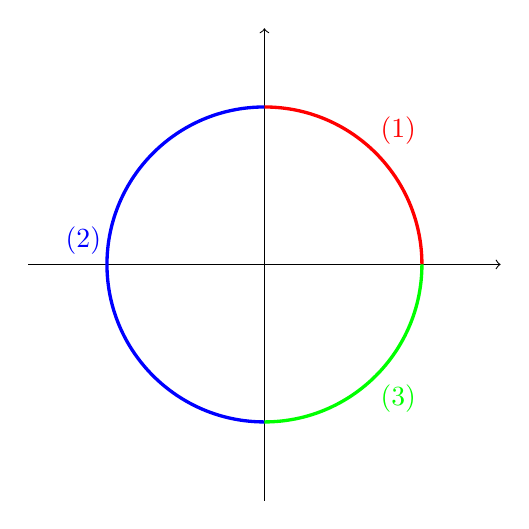
\begin{tikzpicture}[scale=1]
% Ejes
\draw[->] (-3,0) -- (3,0);
\draw[->] (0,-3) -- (0,3);

% Partes de la circunferencia
\draw[very thick,red] (2,0) arc (0:90:2);
\draw[very thick,blue] (0,2) arc (90:270:2);
\draw[very thick,green] (0,-2) arc(270:360:2);

% Etiquetas
\node[red] at (1.7, 1.7) {(1)};
\node[blue] at (-2.3, 0.3) {(2)};
\node[green] at (1.7, -1.7) {(3)};
\end{tikzpicture}
\caption{Circunferencia definida en tres trozos}
\label{imgCirc}
\end{center}
\end{figure}


\[f(x,y,z) =\left\{ \begin{matrix}
Si & (x,y,z) \in 1 &\implies &arcsen\left(\frac{z}{r}\right)\\
Si & (x,y,z) \in 2 &\implies &\displaystyle\frac{\alpha + arcsen\left(\frac{z}{r}\right)}{2} = \frac{\pi}{2}\\
Si & (x,y,z) \in 3 &\implies & \alpha = arcsen\left(\frac{z}{r}\right) + 2\pi
\end{matrix}\right.
\]

Ahora tenemos que estudiar la continuidad des esta función. (Ejercicio para el lector)


\subparagraph{$T_{\ga}M$}

En este caso (al tratarse de una diferencial) tendremos que hallar la imagen de $D\Phi$.

Ejercicio propuesto: $T_{\left(\frac{\pi}{2},\frac{\pi}{2}\right)}M$.


\begin{problem}[4.4]
Sea $\sigma(t) = \left( cos(t),sen(t),t^2(2\pi - t)^2\right), t \in [0,2\pi]$.
\solution
Siempre hemos hablado de parametrizaciones es espacios abiertos, para asegurar la condición de homeomorfismo en casos como este, en el que los puntos cerca de $0$, la inversa me los lleva a puntos lejanos si nos acercamos a $0$ por el $0$ o por el $2\pi$.

Posibles soluciones
\begin{itemize}
\item  Trabajar con el intervalo abierto, pero entonces... el punto $(1,0,0)$ que es el que nos piden no pertenece. ¿Cómo calcular el espacio tangente en $(1,0,0)$? Podríamos hacer los "límites laterales" y calcular el $T_{(1^{-},0,0)}M, T_{(1^{+},0,0)}$ por decirlo de alguna manera y si coinciden, ese tiene que ser el hiperplano tangente en el punto $(1,0,0)$.

\item Definir otro intervalo en el que trabajar. 

Con el $sen$ y $cos$ no tenemos problema porque son periódicas y podríamos trabajar en $\left(\frac{\pi}{2},\frac{\pi}{2}\right)$ pero con la tercera coordenada es más problemático porque no es periódica. Es de la forma:

%\easyimg{imgs/TercCoor.png}{TercCoor}{lblTercCoor}

Idea: 
\begin{itemize}
\item Escribir la extensión $2\pi$ periódica al intervalo $[-2\pi,2\pi]$.
\item Tomar $\tilde{\sigma}(t) = (cos(t),sen(t),\tilde{z}(t)), t\in (-\pi,\pi)$
\end{itemize}
\end{itemize}

\end{problem}
